% !TEX encoding = UTF-8
% !TEX TS-program = pdflatex
% !TEX root = ../tesi.tex

%**************************************************************
\chapter{Descrizione dello stage}
\label{cap:descrizione-stage}
%**************************************************************

\intro{Tale capitolo riporta una descrizione dei possibili rischi, la modalità di svolgimento, le problematiche da risolvere e le soluzioni proposte dell'attività di stage svolta. Viene inoltre riportata la pianificazione del lavoro e gli obiettivi da raggiungere al termine della stessa.}\\

%**************************************************************
\section{Analisi dei rischi}
Al fine di evitare rallentamenti dei periodi di lavoro è stata effettuata una breve analisi dei rischi, in modo da evitare le situazioni che portano alla creazione di eventi non pianificati, ove possibile. I rischi analizzati sono divisi per area di competenza, e per ognuno di essi è mostrata brevemente la strategia di mitigazione.
\begin{itemize}
    \item Livello tecnologico: 
        \begin{itemize}
            \item \textbf{Guasti hardware:} durante lo svolgimento dello stage è possibile che la strumentazione utilizzata, in particolare i computer assegnati, possano incorrere in guasti hardware, rischiando così di causare rallentamenti e perdita del lavoro.
            \\
            Per evitare questo evento verrà regolarmente caricato il materiale su una directory di uno dei server dell'azienda;
            
            \item \textbf{Linguaggio di programmazione poco padroneggiato:} durante lo svolgimento dello stage è richiesto l'utilizzo di \emph{PHP}\glsfirstoccur, linguaggio che non ho usato spesso nella mia carriera universitaria. Questo fatto potrebbe portare a ritardi o a difficoltà nello svolgimento del progetto. 
            \\
            Per far fronte a tale problematica studierò autonomamente le basi del linguaggio per poter affrontare con meno difficoltà il primo periodo di codifica;
            
            \item \textbf{Framework aziendale sconosciuto:} l'utilizzo di un \emph{framework}\glsfirstoccur realizzato da Gestiware S.r.l. e a me completamente sconosciuto potrebbe portare a ritardi o a difficoltà nello svolgimento del progetto.
            \\
             Tuttavia, grazie al periodo di apprendimento pianificato nella prima fase dello stage, e grazie alla presenza di personale esperto con cui confrontarsi, questo rischio non dovrebbe presentarsi;
        \end{itemize}
    \item Livello dei requisiti:
        \begin{itemize}
            \item \textbf{Incomprensioni e scelte non ottimali:} può accadere che alcune attività da svolgere siano fraintese o valutate erroneamente, causando la realizzazione di un prodotto non consono alle aspettative dell'azienda. Per mitigare questo rischio, ogni giorno avviene un incontro con il tutor aziendale per valutare il lavoro svolto e chiarire eventuali dubbi.
        \end{itemize}
\end{itemize}



%**************************************************************
\section{Modalità di svolgimento}
L’attività di stage è stata svolta presso la sede dell'azienda per favorire l’interazione dello studente con il tutor e per affacciarlo alla realtà di un team di sviluppo aziendale.\\
È stata quindi data la possibilità di relazionarsi con professionisti esperti ed essere supportato al meglio in caso di problematiche di realizzazione del progetto e di confrontarsi con il tutor per qualsiasi problematica.\\
L’organizzazione settimanale del lavoro è stata invece gestita tramite dei meeting, sempre con il tutor aziendale, atti a definire lo stato di avanzamento delle attività assegnate e rivedere in tempo reale gli obiettivi settimanali raggiunti o da raggiungere.\\
I risultati sono stati valutati mensilmente in base alla quantità di requisiti soddisfatti e alla qualità del prodotto realizzato.\\
L’orario lavorativo è stato il seguente: dal lunedì al venerdì, dalle 8:30 alle 18:00, con pausa pranzo dalle 12:30 alle 14:00.

%**************************************************************
\section{Pianificazione del lavoro}
La seguente sezione mostra, mediante \emph{diagramma di Gantt}\glsfirstoccur, la distribuzione temporale di ogni singola attività svolta durante il periodo di stage.

\begin{figure}[!h] 
    \centering 
    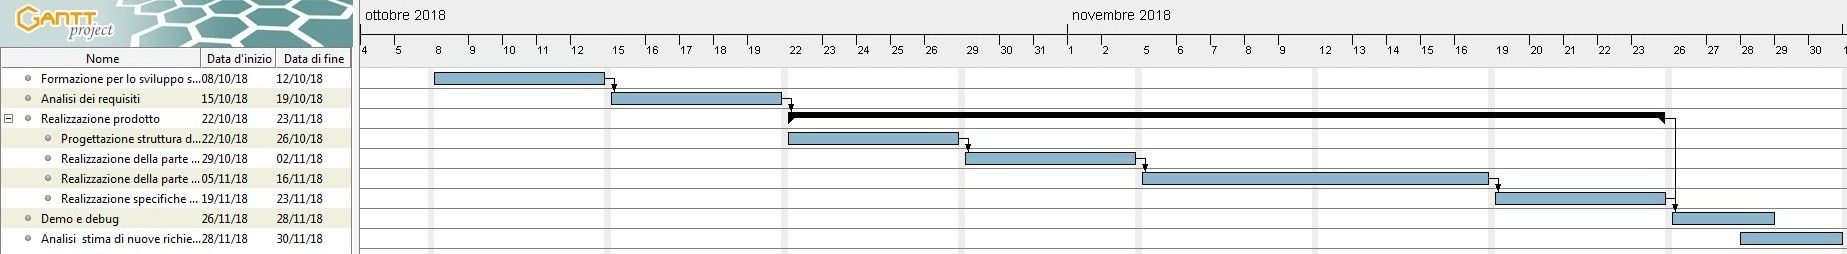
\includegraphics[width=1\columnwidth]{immagini/gantt.png} 
    \caption{Diagramma di Gantt - Attività svolte}
\end{figure}
%**************************************************************
\section{Problema della proponente}
In seguito all'incontro svoltosi in data 6 marzo tra i responsabili di Gestiware S.r.l e il responsabile dell'azienda proponente (Il nome dell'azienda o del responsabile non verranno mai citati per motivi di privacy) è risaltata l'esigenza di quest'ultima di avere un applicativo web in grado di gestire i protocolli in ingresso ed in uscita presso la suddetta. 
\\
Con "gestione di protocolli" si intende tutta l'attività svolta dagli operatori sui documenti in ingresso ed in uscita dall'azienda stessa.
\\
Le principali attività da svolgere sono:
\begin{itemize}
    \item Protocollare il documento, ossia:
        \begin{itemize}
            \item assegnare un identificativo univoco alfanumerico;
            
            \item assegnare un registro di appartenenza per una facile archiviazione;
            
            \item assegnare il documento ad un proprietario.
        \end{itemize}
    \item Smistare il documento al personale interno o anche esterno.
\end{itemize}
Questo tipo di operazioni vengono svolte, per ora, con diversi passaggi manuali, con la scrittura di mail con allegati precedentemente scansionati e/o salvati; quello che manca è un'automatizzazione di questi passaggi e un iter omogeneo che tracci tutto lo storico del protocollo.
\\
È stata inoltre esposta l'esigenza di gestire la privacy dei protocolli in quanto al suo interno sono contenuti dati sensibili di persone e/o aziende. 
%**************************************************************

\section{Analisi dei requisiti}
Tenuto conto dei vincoli elencati nei punti precedenti, per prima cosa si è eseguita un'analisi dei requisiti. Per fare ciò, è stata effettuata una fase di \emph{brainstorming}\glsfirstoccur, congiuntamente con il tutor aziendale, per stabilire quali fossero le feature da implementare e che priorità avrebbe dovuto avere ognuna di esse. Dopo questo primo brainstorming, lo stagista ha proceduto alla stesura del documento di analisi dei requisiti, iniziando con la realizzazione dei diagrammi \emph{UML}\glsfirstoccur che descrivessero tramite casi d'uso le interazioni dell'utente con il sistema.

\subsection{Funzionalità del prodotto}
Le funzionalità principali che l'applicativo web deve avere sono:
\begin{itemize}
        \item solo gli utenti dotati di credenziali di accesso potranno avere accesso all'applicazione web;
        
        \item ad un utente base è consentita la gestione dei protocolli da lui inseriti e a lui assegnati;
        
        \item ad un supervisore è consentita la gestione di tutti i protocolli;
        
        \item si dovrà fornire la possibilità di protocollare un documento in ingresso o in uscita, ossia assegnarne un identificativo, un registro di appartenenza e un "proprietario";
        
        \item deve essere possibile la registrazione di un nuovo contatto;
        
        \item deve esserci la possibilità di stampare il registro dei protocolli;

        \item deve esserci la possibilità di filtrare la lista di protocolli mediante tutti i campi visibili;
        
        \item deve esserci la possibilità di filtrare la lista di protocolli mediante l'utilizzo di scanner di barcode;
        
        \item deve esserci la possibilità di smistare mediante mail i protocolli;

        \item deve esserci la possibilità di inserire commenti e di avere lo storico delle attività;
        
        \item deve esserci la possibilità di configurare le tipologie di protocolli.
    \end{itemize}

\subsection{Casi d'uso}
\subsubsection{Classificazione dei casi d'uso}
Ogni caso d'uso sarà rappresentato con il seguente formalismo:
\begin{center}
    \textbf{UC[Codice]}
\end{center}
dove:\\
\textbf{Codice}: è un numero che identifica in modo univoco i casi d'uso.\\\\
Ogni caso d'uso, inoltre, deve essere descritto secondo la seguente specifica:
\begin{itemize}
    \item
    \textbf{ID}: è il codice identificativo del caso d'uso, di cui il formalismo sopra;
    \item
    \textbf{Attori}: gli attori coinvolti, sia principali sia secondari;
    \item
    \textbf{Descrizione}: breve descrizione del caso d'uso;
    \item
    \textbf{Pre-condizioni}: lo stato in cui si deve trovare il sistema affinché si verifichino le post-condizioni;
    \item
    \textbf{Post-condizioni}: le istruzioni che risultano vere dopo il verificarsi degli eventi del caso d'uso;
    \item
    \textbf{Scenario principale}: rappresenta il flusso principale degli eventi come elenco di azioni tra l'utente e il sistema;
    \item
    \textbf{Scenari alternativi}: casi d'uso esterni al flusso principale degli eventi che servono a gestire eventuali eccezioni o errori.
\end{itemize}
\newpage


\subsubsection{UC1 - Login}
    \label{UC1}
    \begin{figure}[!h] 
        \centering 
        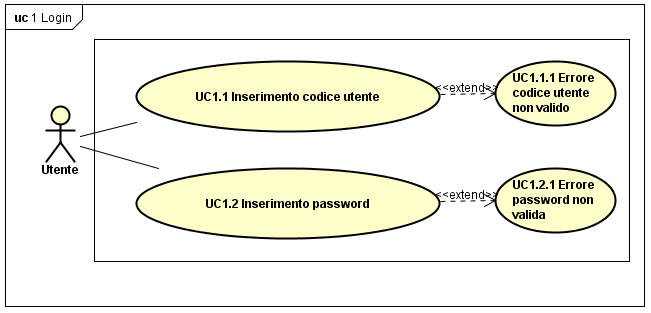
\includegraphics[width = 13cm]{immagini/UseCase/login.png} 
        \caption{UC1 Login}
    \end{figure}
    \textbf{Attori primari:} Utente non autenticato.
    \\
    \\
    \textbf{Descrizione:} L'attore vuole accedere al sistema.
    \\
    \\
    \textbf{Precondizione:} Il sistema visualizza il form per l'inserimento delle credenziali utente.
    \\
    \\
    \textbf{Postcondizione:}Il sistema ha autenticato l'attore, che viene rimandato alla pagina iniziale come utente autenticato.
    \\
    \\
    \textbf{Scenario principale:}
        \begin{itemize}
            \item L'attore deve inserire l'email (\hyperref[UC1.1]{UC1.1});
            \item L'attore deve inserire la password (\hyperref[UC1.2]{UC1.2});
        \end{itemize}
    \textbf{Scenari alternativi:} Il sistema visualizza un messaggio di errore relativo all'inserimento dei dati.


\subsubsection{UC1.1 - Inserimento codice utente}
    \label{UC1.1}
    \textbf{Attori primari:} Utente non autenticato.
    \\
    \\
    \textbf{Descrizione:} L'attore inserisce il proprio codice utente.
    \\
    \\
    \textbf{Precondizione:} Il sistema visualizza un campo in cui inserire il codice utente.
    \\
    \\
    \textbf{Postcondizione:} Il sistema ha l'informazione relativa all'utente.
    \\
    \\
    \textbf{Scenario principale:} L'attore deve inserire il proprio codice utente nell'apposita casella di testo.


\subsubsection{UC1.2 - Inserimento password}
    \label{UC1.2}
    \textbf{Attori primari:} Utente non autenticato.
    \\
    \\
    \textbf{Descrizione:} L'attore inserisce la propria password.
    \\
    \\
    \textbf{Precondizione:} Il sistema visualizza un campo in cui inserire la password.
    \\
    \\
    \textbf{Postcondizione:} Il sistema ha l'informazione relativa alla password.
    \\
    \\
    \textbf{Scenario principale:} L'attore deve inserire la propria password nell'apposita casella di testo.
    
    
    \subsubsection{UC1.3 - Errore "Email o Password errati"}
    \textbf{Attori primari:} Utente non autenticato.
    \\
    \\
    \textbf{Descrizione:} Il sistema visualizza un opportuno messaggio di errore relativo ai dati errati inseriti dall'attore.
    \\
    \\
    \textbf{Precondizione:} L'attore ha richiesto di effettuare la login tramite i propri dati.
    \\
    \\
    \textbf{Postcondizione:} Il sistema nega l'autenticazione visualizzando un messaggio di errore relativo ai dati inseriti.
    \\
    \\
    \textbf{Scenario principale:} Il sistema nega il login visualizzando un messaggio di errore relativo ai dati errati inseriti dall'attore.
    
    \newpage
    \subsubsection{UC}
    \label{UC}
    \begin{figure}[!h] 
        \centering 
        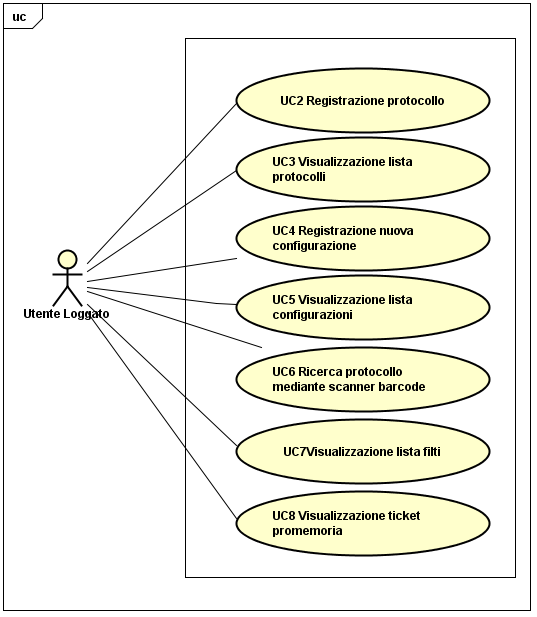
\includegraphics[width = 11cm]{immagini/UseCase/postlogin.png}
        \caption{UC Post Login}
    \end{figure}
    
    \textbf{Attori primari:} Utente loggato.
    \\
    \\
    \textbf{Descrizione:} L'utente loggato ha accesso a molteplici funzionalità.
    \\
    \\
    \textbf{Precondizione:} L'utente ha accesso al sistema.
    \\
    \\
    \textbf{Postcondizione:} Il sistema ha permesso di gestire le funzionalità di interesse dall'utente che si interfaccia con esso.
    \\
    \\
    \textbf{Scenario principale:} L'attore una volta autenticato può visualizzare le seguenti funzionalità:
            \begin{itemize}
                \item registrazione protocollo;
                \item Visualizzazione lista protocolli;
                \item registrazione nuova configurazione;
                \item visualizzazione lista configurazioni;
                \item ricerca protocollo mediante scanner di barcode;
                \item visualizzazione filtri;
                \item visualizzazione ticket promemoria.
            \end{itemize}

\subsubsection{UC2 Registrazione protocollo}
    \label{UC2}
    \begin{figure}[!h] 
        \centering 
        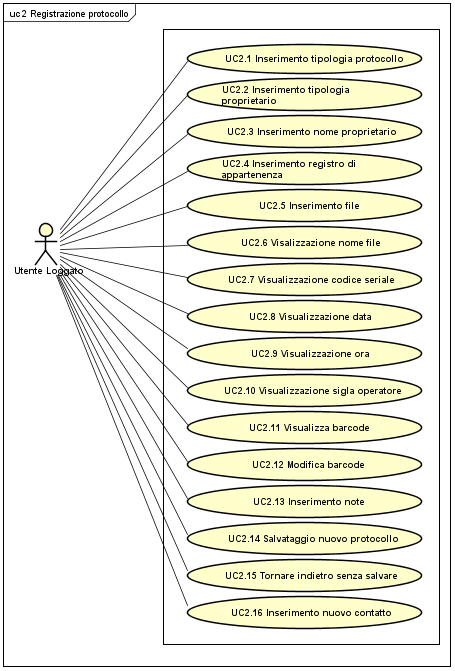
\includegraphics[width = 11cm]{immagini/UseCase/registrazioneprotocollo.png}
        \caption{UC2 Registrazione protocollo}
    \end{figure}
    
    \textbf{Attori primari:} Utente loggato.
    \\ 
    \\
    \textbf{Descrizione:} L'utente può registrare un nuovo protocollo compilando l'apposito form.
    \\
    \\
    \textbf{Precondizione:} L'utente ha accesso al form di registrazione di un nuovo protocollo.
    \\
    \\
    \textbf{Postcondizione:} Il sistema salva il protocollo regitrato mediante apposito form.
    \\
    \\
    \textbf{Scenario principale:} L'utente per registrare il nuovo protocollo deve inserire le seguenti informazioni o compiere le seguenti azioni:
            \begin{itemize}
                \item tipologia protocollo;
                \item tipologia proprietario;
                \item nome proprietario;
                \item registro di appartenenza ;
                \item file del documento da protocollare;
                \item nome del file;
                \item codice seriale del protocollo;
                \item data di registrazione;
                \item ora di registrazione;
                \item sigla operatore;
                \item barcode;
                \item modificare il codice a barre;
                \item salvare il protocollo;
                \item annullare la registrazione;
                \item inserire un nuovo contatto.
            \end{itemize}

\subsubsection{UC2.1 - Inserimento tipologia protocollo}
    \label{UC2.1}
    \textbf{Attori primari:} Utente loggato.
    \\
    \\
    \textbf{Descrizione:} Una volta selezionata una tipologia verranno stampati a video i campi \emph{metadato }\glsfirstoccur inseriti in fase di configurazione della tipologia.
    \\
    \\
    \textbf{Precondizione:} Il sistema visualizza un campo \textit{select} dove tutte le option sono le tipologie create dall'utente in \hyperref[UC4]{UC4}.
    \\
    \\
    \textbf{Postcondizione:} Il sistema stampa a video i campi metadato associati alla tipologia selezionata.
    \\
    \\
    \textbf{Scenario principale:} L'attore deve compilare tutti i campi metadato marcati come \textit{required}.
\newpage

\subsubsection{UC2.16 Inserimento nuovo contatto}
    \label{UC2.16}
    \begin{figure}[!h] 
        \centering 
        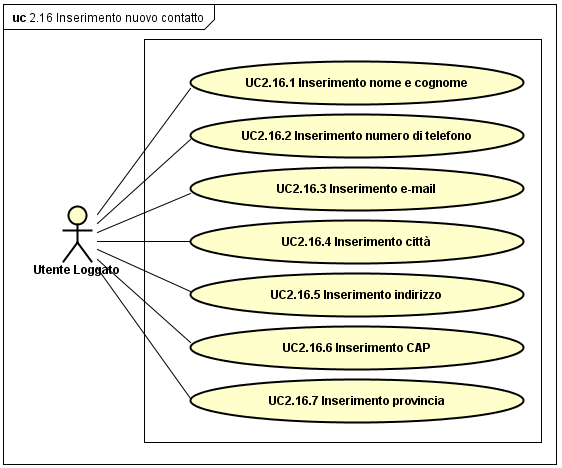
\includegraphics[width = 11cm]{immagini/UseCase/inserimentocontatto.png}
        \caption{UC2.16 Inserimento nuovo contatto}
    \end{figure}
    
    \textbf{Attori primari:} Utente loggato.
    \\ 
    \\
    \textbf{Descrizione:} L'utente se vuole assegnare il protocollo ad un proprietario non registrato nel database può registrarne uno nuovo con apposito form.
    \\
    \\
    \textbf{Precondizione:} L'utente seleziona "nuovo contatto" nella \textit{select} dedicata alla tipologia di proprietario.
    \\
    \\
    \textbf{Postcondizione:} Il sistema stampa a schermo il form di registrazione di un nuovo contatto.
    \\
    \\
    \textbf{Scenario principale:} L'utente per registrare il nuovo contatto deve inserire le seguenti informazioni:
            \begin{itemize}
                \item nome e cognome del contatto;
                \item numero di telefono del contatto;
                \item indirizzo e-mail;
                \item città;
                \item indirizzo;
                \item CAP;
                \item Provincia.
            \end{itemize}

\subsubsection{UC3 Visualizzazione lista protocolli}
    \label{UC3}
    \textbf{Attori primari:} Utente loggato.
    \\
    \\
    \textbf{Descrizione:} L'utente visualizza una lista di tutti i protocolli che deve visionare.
    \\
    \\
    \textbf{Precondizione:} Il sistema pende dal database tutti i protocolli di interesse.
    \\
    \\
    \textbf{Postcondizione:} Il sistema stampa a video tutti i protocolli.
    \\
    \\
    \textbf{Scenario principale:} L'attore può aprire uno qualsiasi dei protocolli della lista.
    \newpage

\subsubsection{UC3.1 Visualizzazione singolo protocollo}
    \label{UC3.1}
    \begin{figure}[!h] 
        \centering 
        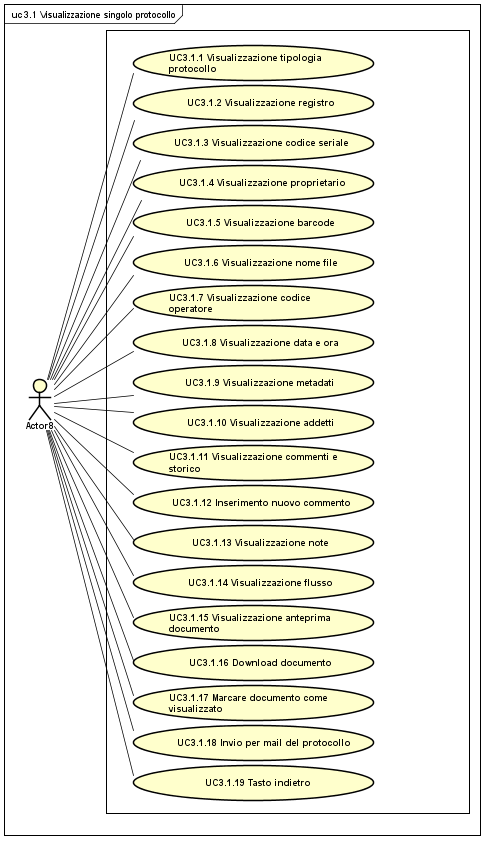
\includegraphics[width = 11cm]{immagini/UseCase/dettaglioprotocollo.png}
        \caption{UC3.1 Visualizzazione singolo protocollo}
    \end{figure}
    
    \textbf{Attori primari:} Utente loggato.
    \\ 
    \\
    \textbf{Descrizione:} L'utente apre la pagina di dettaglio di un singolo protocollo e ne visualizza le informazioni.
    \\
    \\
    \textbf{Precondizione:} L'utente seleziona uno dei protocolli nella lista descritta in \hyperref[UC3]{UC3}.
    \\
    \\
    \textbf{Postcondizione:} Il sistema stampa a schermo le informazioni riguardanti il protocollo selezionato dall'utente.
    \\
    \\
    \textbf{Scenario principale:} L'utente può:
            \begin{itemize}
                \item visualizzare la tipologia protocollo;
                \item visualizzare il registro di appartenenza;
                \item visualizzare il codice seriale;
                \item visualizzare il proprietario a cui è intestato il protocollo;
                \item visualizzare il barcode;
                \item visualizzare il nome file;
                \item visualizzare il codice operatore;
                \item visualizzare la data e ora;
                \item visualizzare i metadati corrispondenti alla tipologia;
                \item visualizzare gli operatori addetti all'elaborazione della tipologia di cui fa parte il protocollo;
                \item visualizzare i commenti e lo storico del protocollo;
                \item inserire un nuovo commento;
                \item visualizzare le note riguardanti il protocollo;
                \item visualizzare il flusso del protocollo;
                \item visualizzare l'anteprima del documento caricato;
                \item premere il tasto download documento;
                \item premere il tasto per marcare come visionato un protocollo;
                \item premere il tasto per inviare via mail il protocollo.
            \end{itemize}
        \newpage
        
\subsubsection{UC3.1.18 Invio per mail del protocollo}
    \label{UC3.1.18}
    \begin{figure}[!h] 
        \centering 
        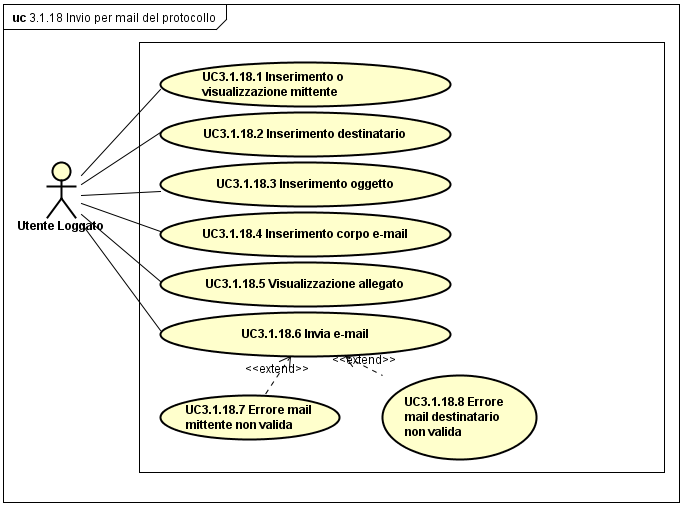
\includegraphics[width = 15cm]{immagini/UseCase/inviomail.png}
        \caption{UC3.1.18 Invio per mail del protocollo}
    \end{figure}
    
    \textbf{Attori primari:} Utente loggato.
    \\ 
    \\
    \textbf{Descrizione:} L'utente facendo \textit{click} sul tasto "Invia" citato in \hyperref[UC3.1]{UC3.1} accederà ad un form di compilazione ed invio di una e-mail.
    \\
    \\
    \textbf{Precondizione:} L'utente seleziona uno dei protocolli nella lista descritta in \hyperref[UC3]{UC3}.
    \\
    \\
    \textbf{Postcondizione:} Il sistema stampa a schermo il form di compilazione della mail.
    \\
    \\
    \textbf{Scenario principale:} L'utente deve inserire le seguenti informazioni per proseguire con l'invio della mail:
            \begin{itemize}
                \item mittente;
                \item destinatario;
                \item oggetto;
                \item corpo della e-mail;
                \item allegato;
                \item premere tasto "Invia" per inviare la mail.
            \end{itemize}
            

\subsubsection{UC4 Registrazione nuova configurazione}
    \label{UC4}
    \begin{figure}[!h] 
        \centering 
        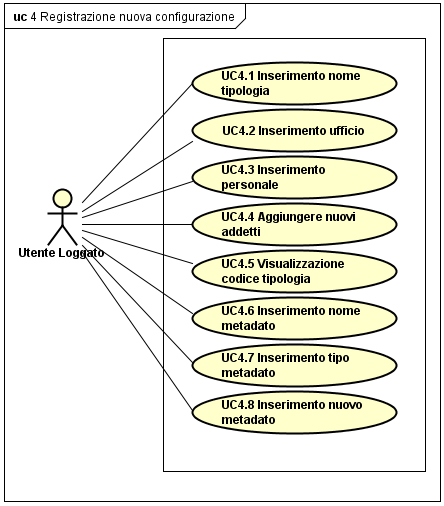
\includegraphics[width = 11cm]{immagini/UseCase/regnuovaconfig.png}
        \caption{UC4 Registrazione nuova configurazione}
    \end{figure}
    
    \textbf{Attori primari:} Utente loggato.
    \\ 
    \\
    \textbf{Descrizione:} L'utente è in grado di creare una nuova tipologia di documento.
    \\
    \\
    \textbf{Precondizione:} L'utente ha accesso all'apposita sezione del sito web.
    \\
    \\
    \textbf{Postcondizione:} Il sistema stampa a schermo il form di compilazione per registrare una nuova tipologia.
    \\
    \\
    \textbf{Scenario principale:} L'utente può:
            \begin{itemize}
                \item inserire nome tipologia;
                \item inserire nome ufficio;
                \item inserire personale dell'ufficio selezionato a cui attribuire l'elaborazione dei futuri protocolli;
                \item aggiungere nuovi addetti;
                \item visualizzare il codice attribuito alla tipologia in fase di creazione;
                \item inserire il nome di un metadato.
                \item inserire il tipo del metadato precedente;
                \item inserire un nuovo metadato.
            \end{itemize}
            
\subsubsection{UC4.4 Aggiungere nuovi addetti}
    \label{UC4.4}
    \textbf{Attori primari:} Utente loggato.
    \\
    \\
    \textbf{Descrizione:} L'utente premendo il tasto "Aggiungi" sito accanto alla selezione dell'ufficio e del personale aggiungerà una nuova riga dove poter selezionare un nuovo ufficio e dei nuovi addetti.
    \\
    \\
    \textbf{Precondizione:} L'utente seleziona "Aggiungi".
    \\
    \\
    \textbf{Postcondizione:} Il sistema stampa a video una nuova riga dove poter selezionare un nuovo ufficio e dei nuovi addetti.
    \\
    \\
    \textbf{Scenario principale:} L'attore può:
        \begin{itemize}
                \item inserire ufficio;
                \item inserire personale addetto;
            \end{itemize}
            
\subsubsection{UC4.8 Inserimento nuovo metadato}
    \label{UC4.8}
    \textbf{Attori primari:} Utente loggato.
    \\
    \\
    \textbf{Descrizione:} L'utente premendo il tasto "Aggiungi" sito accanto ai campi di inserimento di un metadato aggiungerà una nuova riga dove poter inserire il nome di un nuovo metadato e il tipo dello stesso.
    \\
    \\
    \textbf{Precondizione:} L'utente seleziona "Aggiungi".
    \\
    \\
    \textbf{Postcondizione:} Il sistema stampa a video una nuova riga dove poter inserire nome e tipo di un nuovo metadato.
    \\
    \\
    \textbf{Scenario principale:} L'attore può:
        \begin{itemize}
            \item inserire un nuovo metadato;
            \item inserire il tipo del nuovo metadato;
        \end{itemize}
        
\subsubsection{UC5 Visualizzazione lista delle configurazioni}
    \label{UC5}
    \textbf{Attori primari:} Utente loggato.
    \\
    \\
    \textbf{Descrizione:} L'utente visualizza una lista di tutti i protocolli che deve visionare.
    \\
    \\
    \textbf{Precondizione:} Il sistema pende dal database tutte le configurazioni esistenti.
    \\
    \\
    \textbf{Postcondizione:} Il sistema stampa a video tutte le configurazioni
    \\
    \\
    \textbf{Scenario principale:} L'attore può aprire la pagina dedicata alla visualizzazione delle informazioni riguardanti una singola tipologia di protocollo.
    
\subsubsection{UC5.1 Visualizzazione singola configurazione}
    \label{UC5.1}
    \begin{figure}[!h] 
        \centering 
        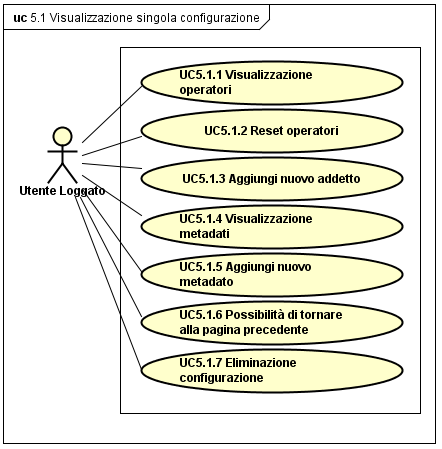
\includegraphics[width = 11cm]{immagini/UseCase/dettaglioconfig.png}
        \caption{UC5.1 Visualizzazione singola configurazione}
    \end{figure}
    
    \textbf{Attori primari:} Utente loggato.
    \\ 
    \\
    \textbf{Descrizione:} L'utente può visualizzare, modificare o eliminare le informazioni relative ad una tipologia.
    \\
    \\
    \textbf{Precondizione:} L'utente ha accesso all'apposita sezione del sito web.
    \\
    \\
    \textbf{Postcondizione:} Il sistema stampa a schermo le informazioni riguardanti una singola tipologia.
    \\
    \\
    \textbf{Scenario principale:} L'utente può:
            \begin{itemize}
                \item visualizzare gli operatori addetti;
                \item resettare la configurazione degli operatori;
                \item aggiungere un nuovo addetto
                \item visualizzare i metadati;
                \item aggiungere un nuovo metadato;
                \item tornare alla pagina precedente;
                \item eliminare una configurazione.
            \end{itemize}
%***************************************************************
\newpage
\subsection{Requisiti}

\subsubsection{Classificazione dei requisiti}
Ogni requisito sarà rappresentato con il seguente formalismo:
\begin{center}
    \textbf{R[Tipo][Utilità][Codice]}
\end{center}
dove:
\begin{itemize}
	\item
	\textbf{Tipo}: indica se il requisito è di tipo
	\begin{itemize}
	    \item \textbf{F}: indica un requisito di funzionale;
	    \item \textbf{Q}: indica un requisito di qualitativo;
	    \item \textbf{V}: indica un requisito di vincolo.
	\end{itemize}
	\item
	\textbf{Utilità}: può assumere i seguenti valori
	\begin{itemize}
	    \item \textbf{O (obbligatorio)}: questi requisiti dovranno necessariamente essere soddisfatti, in quanto di importanza fondamentale per la riuscita del progetto;
	    \item \textbf{D (desiderabile)}: questi requisiti non sono ritenuti fondamentali per la riuscita del progetto, tuttavia un loro soddisfacimento è percepito come desiderabile;
	    \item \textbf{F (facoltativo)}: il soddisfacimento di questi requisiti risulta del tutto facoltativo.
	\end{itemize}
	\item
	\textbf{Codice}: deve identificare in modo univoco ogni requisito. Per le gerarchie di requisiti, questo codice è nel formato [Codice padre].[Codice figlio].
\end{itemize}

\subsubsection{Requisiti funzionali}
Di seguito si riporta la tabella contenente tutti i requisiti funzionali individuati, comprensiva di descrizione del requisito, tracciamento dell'UC fonte dal quale esso ha origine (nel caso il requisito non sia stato descritto in un caso d'uso, verrà indicata come fonte "decisione interna") e stato di completamento raggiunto al termine dello stage (Completato/Non completato).
    \renewcommand{\arraystretch}{1.5}%
    \begin{longtable}{| p{3cm} | p{6cm} | p{3cm} | p{3cm} |}
        \caption[Requisiti Funzionali]{Requisiti Funzionali}
        \label{tabella:req0}
        \endlastfoot
        \hline
        \textbf{Requisito} & \textbf{Descrizione} & \textbf{fonte} & \textbf{Stato}\\
        \hline
        \endhead
        RFO1 & L'attore può accedere al sistema tramite login. & UC1 & Completato
        \\ \hline
        
        RFO1.1 & L'attore deve poter inserire il proprio codice utente. & UC1.1 & Completato
        \\ \hline
        
        RFO1.1.1 & L'attore deve poter visualizzare un messaggio d'errore qualora il codice utente sia sbagliato. & UC1.1.1 & Completato
        \\ \hline
        
        RFO1.2 & L'attore deve poter inserire la propria password & UC1.2 & Completato
        \\ \hline
        
        RFO1.2.1 & L'attore deve poter visualizzare un messaggio d'errore qualora la password sia sbagliata. & UC1.2.1 & Completato
        \\ \hline
        
        RFO2 & Deve essere possibile protocollare un documento & UC2 & Completato
        \\ \hline
        
        RFD1 & Deve essere possibile selezionare una tipologia di documento & UC2.1 & Completato
        \\ \hline
        
        RFO2.1 & Deve essere possibile selezionare la tipologia di un proprietario & UC2.2 & Completato
        \\ \hline
        
        RFO2.2 & Deve essere possibile inserire il nome del proprietario del protocollo & UC2.3 & Completato
        \\ \hline
        
        RFD2 & Deve essere possibile visualizzare i suggerimenti relativi al nome del proprietario & UC2.3 & Completato
        \\ \hline
        
        RFO2.3 & Deve essere possibile selezionare il registro di appartenenza & UC2.4 & Completato
        \\ \hline
        
        RFO2.4 & Al cambiare del registro di appartenenza deve essere stampato il rispettivo codice & UC2.4 e UC2.7 & Completato
        \\ \hline
        
        RFO2.5 & Deve essere possibile caricare un file & UC2.5 & Completato
        \\ \hline
        
        RFD3 & Deve essere possibile visualizzare il nome del file una volta caricato un documento & UC2.6 & Completato
        \\ \hline
        
        RFO2.6 & Deve essere possibile visualizzare il codice seriale univoco & UC2.7 & Completato
        \\ \hline
        
        RFO2.7 & Deve essere possibile visualizzare la data per la registrazione del protocollo & UC2.8 & Completato
        \\ \hline
        
        RFO2.8 & Deve essere possibile visualizzare l'ora per la registrazione del protocollo & UC2.9 & Completato
        \\ \hline
        
        RFO2.9 & Deve essere possibile visualizzare il codice dell'operatore che sta eseguendo la registrazione del protocollo & UC2.10 & Completato
        \\ \hline
        
        RFO2.10 & Deve essere possibile visualizzare un codice barcode univoco per il protocollo & UC2.11 & Completato
        \\ \hline
        
        RFO2.11 & Deve essere possibile modificare il barcode proposto dal sistema & UC2.12 & Completato
        \\ \hline
        
        RFD4 & Deve essere possibile inserire delle note & UC2.13 & Completato
        \\ \hline
        
        RFO2.12 & Deve essere possibile salvare il protocollo in inserimento & UC2.14 & Completato
        \\ \hline
        
        RFD5 & Deve essere possibile tornare indietro mediante bottone senza salvare il protocollo in elaborazione & UC2.15 & Completato
        \\ \hline
        
        RFO2.13 & Deve essere possibile inserire un nuovo contatto come proprietario del protocollo & UC2.16 & Completato
        \\ \hline
        
        RFO2.13.1 & Deve essere possibile inserire nome e cognome di un nuovo contatto & UC2.16.1 & Completato
        \\ \hline
        
        RFO2.13.2 & Deve essere possibile inserire un numero di telefono del nuovo contatto & UC2.16.2 & Completato
        \\ \hline
        
        RFO2.13.3 & Deve essere possibile inserire una e-mail del nuovo contatto & UC2.16.3 & Completato
        \\ \hline
        
        RFO2.13.4 & Deve essere possibile inserire la città di provenienza del nuovo contatto & UC2.16.4 & Completato
        \\ \hline
        
        RFO2.13.5 & Deve essere possibile inserire l'indirizzo del nuovo contatto & UC2.16.5 & Completato
        \\ \hline
        
        RFO2.13.6 & Deve essere possibile inserire il CAP del nuovo contatto & UC2.16.6 & Completato
        \\ \hline
        
        RFO2.13.7 & Deve essere possibile inserire la provincia del nuovo contatto & UC2.16.7 & Completato
        \\ \hline
        
        RFO3 & L'attore, in base ai suoi permessi, dovrà visualizzare la lista dei protocolli & UC3 & Completato
        \\ \hline
        
        RFO3.1 & Deve essere possibile visualizzare il singolo protocollo & UC3.1 & Completato
        \\ \hline
        
        RFO3.1.1 & Deve essere possibile visualizzare la tipologia di protocollo & UC3.1.1 & Completato
        \\ \hline
        
        RFO3.1.2 & Deve essere possibile visualizzare il registro di appartenenza del protocollo & UC3.1.2 & Completato
        \\ \hline
        
        RFO3.1.3 & Deve essere possibile visualizzare il codice seriale del protocollo & UC3.1.3 & Completato
        \\ \hline
        
        RFO3.1.4 & Deve essere possibile visualizzare il proprietario del protocollo & UC3.1.4 & Completato
        \\ \hline
        
        RFO3.1.5 & Deve essere possibile visualizzare il barcode assegnato al protocollo & UC3.1.5 & Completato
        \\ \hline
        
        RFO3.1.6 & Deve essere possibile visualizzare il nome del file allegato al protocollo & UC3.1.6 & Completato
        \\ \hline
        
        RFO3.1.7 & Deve essere possibile visualizzare l'operatore che ha provveduto alla registrazione del protocollo & UC3.1.7 & Completato
        \\ \hline
        
        RFO3.1.8 & Deve essere possibile visualizzare la data e l'ora di registrazione del protocollo & UC3.1.8 & Completato
        \\ \hline
        
        RFO3.1.9 & Deve essere possibile visualizzare i metadati del protocollo & UC3.1.9 & Completato
        \\ \hline
        
        RFO3.1.10 & Deve essere possibile visualizzare gli addetti all'elaborazione del protocollo & UC3.1.10 & Completato
        \\ \hline
        
        RFO3.1.11 \label{RFO3.1.11} & Deve essere possibile visualizzare lo storico e i commenti riguardanti il protocollo & UC3.1.11 & Completato
        \\ \hline
        
        RFO3.1.12 & Deve essere possibile inserire nuovi commenti riguardanti il protocollo & UC3.1.12 & Completato
        \\ \hline
        
        RFO3.1.13 & Deve essere possibile visualizzare le note relative al protocollo & UC3.1.13 & Completato
        \\ \hline
        
        RFF1 & Deve essere possibile visualizzare il flusso del protocollo & UC3.1.14 &  Non completato
        \\ \hline
        
        RFO3.1.14 & Deve essere possibile visualizzare l'anteprima del documento allegato al protocollo & UC3.1.15 & Completato
        \\ \hline
        
        RFO3.1.15 & Deve essere possibile scaricare il documento allegato al protocollo & UC3.1.16 & Completato
        \\ \hline
        
        RFO3.1.16 & Deve essere possibile per l'attore marcare come visualizzato il protocollo a lui assegnato & UC3.1.17 & Completato
        \\ \hline
        
        RFO3.1.17 & Deve essere possibile inviare per mail il protocollo & UC3.1.18 & Completato
        \\ \hline
        
        RFO3.1.17.1 & Deve essere possibile inserire o visualizzare il mittente & UC3.1.17.1 & Completato
        \\ \hline
        
        RFO3.1.17.2 & Deve essere possibile inserire il destinatario & UC3.1.17.2 & Completato
        \\ \hline
        
        RFO3.1.17.3 & Deve essere possibile inserire l'oggetto & UC3.1.17.3 & Completato
        \\ \hline
        
        RFO3.1.17.4 & Deve essere possibile inserire il testo della mail & UC3.1.17.4 & Completato
        \\ \hline
        
        RFO3.1.17.5 & Deve essere possibile visualizzare l'allegato caricato automaticamente come tale & UC3.1.17.5 & Completato
        \\ \hline
        
        RFO3.1.17.6 & Deve essere possibile inviare la mail& UC3.1.17.6 & Completato
        \\ \hline
        
        RFO3.1.17.7 & Deve essere possibile visualizzare un errore se l'indirizzo del mittente non è valido & UC3.1.17.7 & Completato
        \\ \hline
        
        RFO3.1.17.8 & Deve essere possibile visualizzare un errore se l'indirizzo del destinatario non è valido & UC3.1.17.8 & Completato
        \\ \hline
        
        RFO4 & Deve essere possibile registrare una nuova configurazione & UC4 & Completato
        \\ \hline
        
        RFO4.1 & Deve essere possibile inserire in nome della nuova tipologia & UC4.1 & Completato
        \\ \hline
        
        RFO4.2 & Deve essere possibile inserire un ufficio addetto all'elaborazione della suddetta tipologia & UC4.2 & Completato
        \\ \hline
        
        RFO4.3 & Deve essere possibile inserire il personale dell'ufficio selezionato & UC4.3 & Completato
        \\ \hline
        
        RFO4.3.1 & Deve essere possibile selezionare tutto il personale dell'ufficio & UC4.3 & Completato
        \\ \hline
        
        RFO4.3.2 & Deve essere possibile selezionare parte del personale dell'ufficio selezionato & UC4.3 & Completato
        \\ \hline
        
        RFO4.4 & Deve essere possibile aggingere una nuova composizione ufficio e personale & UC4.4 & Completato
        \\ \hline
        
        RFO4.4.1 & Deve essere possibile inserire un ufficio addetto all'elaborazione della suddetta tipologia & UC4.4.1 & Completato
        \\ \hline
        
        RFO4.4.2 & Deve essere possibile possibile inserire il personale dell'ufficio selezionato & UC4.4.2 & Completato
        \\ \hline
        
        RFO4.4.2.1 & Deve essere possibile selezionare tutto il personale dell'ufficio & UC4.3 & Completato
        \\ \hline
        
        RFO4.4.2.2 & Deve essere possibile selezionare parte del personale dell'ufficio selezionato & UC4.3 & Completato
        \\ \hline
        
        RFO4.5 & Deve essere possibile visualizzare il codice assegnato alla nuova configurazione & UC4.5 & Completato
        \\ \hline
        
        RFO4.6 & Deve essere possibile inserire il nome del metadato della nuova tipologia & UC4.6 & Completato
        \\ \hline
        
        RFO4.7 & Deve essere possibile inserire il tipo di metadato della nuova tipologia & UC4.7 & Completato
        \\ \hline
        
        RFO4.8 & Deve essere possibile inserire un nuovo metadato alla configurazione & UC4.8 & Completato
        \\ \hline
        
        RFO4.8.1 & Deve essere possibile inserire il nome del metadato della nuova tipologia & UC4.8.1 & Completato
        \\ \hline
        
        RFO4.8.2 & Deve essere possibile inserire il tipo di metadato della nuova tipologia & UC4.8.2 & Completato
        \\ \hline
        
        RFO5 & Deve essere possibile visualizzare la lista delle configurazioni & UC5 & Completato
        \\ \hline
        
        RFO5.1 & Deve essere possibile visualizzare la lista degli operatori addetti e i rispettivi uffici & UC5.1.1 & Completato
        \\ \hline
        
        RFO5.2 & Deve essere possibile resettare la configurazione degli operatori & UC5.1.2 & Completato
        \\ \hline
        
        RFO5.3 & Deve essere possibile aggiungere una nuova configurazione ufficio personale & UC5.1.3 & Completato
        \\ \hline
        
        RFO5.4 & Deve essere possibile visualizzare la lista dei metadati & UC5.1.4 & Completato
        \\ \hline
        
        RFO5.5 & Deve essere possibile aggiungere un nuovo metadato & UC5.1.5 & Completato
        \\ \hline
        
        RFO5.6 & Deve essere possibile tornare indietro senza salvare le modifiche alla configurazione & UC5.1.6 & Completato
        \\ \hline
        
        RFO5.7 & Deve essere possibile eliminare una configurazione qualora non ci siano documenti collegati alla suddetta & UC5.1.7 & Completato
        \\ \hline
        
        RFO6 \label{RFO6} & Deve essere possibile ricercare un protocollo mediante scanner di barcode & UC6 & Completato
        \\ \hline
        
        RFO7 & visualizzare e utilizzare la lista di filtri per la dashboard & UC7 & Completato
        \\ \hline
        
        RFF2 & Deve essere possibile visualizzare il ticket promemoria che ricorda all'utente quanti protocolli sono ancora da visionare  & UC8 & Completato
        \\ \hline
    \end{longtable}
\newpage

\subsubsection{Requisiti di vincolo}
    Di seguito si riporta la tabella contenente tutti i requisiti di vincolo individuati, comprensiva di descrizione del requisito e stato di completamento raggiunto al termine dello stage (Completato/Non completato).
    \renewcommand{\arraystretch}{1.5}%
    \begin{longtable}{| p{3cm} | p{9cm} | p{3cm} |}
        \caption[Requisiti di Vincolo]{Requisiti di Vincolo}
        \label{tabella:req0}
        \endlastfoot
        \hline
        \textbf{Requisito} & \textbf{Descrizione} & \textbf{Stato}\\
        \hline
        \endhead
        RVO1 & La pagina web deve funzionare correttamente su browser Google Chrome dalla versione 49 & Completato 
        \\ \hline
        
        RVO2 & La pagina web deve funzionare correttamente su browser Firefox dalla versione 5 & Completato 
        \\ \hline
        
        RVO3 & La pagina web deve funzionare correttamente su browser Microsoft Edge dalla versione 15 & Completato
        \\ \hline
        
        RVO4 & La pagina web deve funzionare correttamente su browser Safari dalla versione 11 & Completato 
        \\ \hline
    \end{longtable}

\subsubsection{Requisiti di qualità}
    Di seguito si riporta la tabella contenente tutti i requisiti di qualità individuati, comprensiva di descrizione del requisito e stato di completamento raggiunto al termine dello stage (Completato/Non completato).
    \renewcommand{\arraystretch}{1.5}%
    \begin{longtable}{| p{3cm} | p{9cm} | p{3cm} |}
        \caption[Requisiti di Vincolo]{Requisiti di Vincolo}
        \label{tabella:req0}
        \endlastfoot
        \hline
        \textbf{Requisito} & \textbf{Descrizione} & \textbf{Stato}\\
        \hline
        \endhead
        RQO1 & L'interfaccia utente deve essere sviluppata in lingua italiana & Completo
        \\ \hline
        
        RQO2 & Il processo di sviluppo del progetto deve attenersi ai principi qualitativi dell'azienda & Completato
        \\ \hline
        
        RQO3 & Il processo di sviluppo del progetto deve attenersi ai principi qualitativi dell'azienda & Completato
        \\ \hline
        
        RQO4 &  Lo sviluppo del progetto deve avvenire nei tempi previsti dal piano di lavoro & Completato
        \\ \hline
        
        RQD1 &  Deve essere fornita documentazione relativa all'analisi dei requisiti, mockup e struttura del software & Completato
        \\ \hline
    \end{longtable}
    \newpage
\subsubsection{Riepilogo dei requisiti}
    \normalsize
    \renewcommand{\arraystretch}{1.5}%
    \begin{longtable}{| p{3cm} | c | c | c || c |}
        \caption[Riepilogo Requisiti]{Riepilogo Requisiti}
        \label{tabella:riepilogorequi}
        \endlastfoot
        \hline
        \textbf{Tipo} & \textbf{Obbligatorio} & \textbf{Desiderabile} & \textbf{Facoltativo} & Totale\\
        \hline
        Funzionali & 80 & 4 & 2 & 86\\ \hline
        Vincolo & 4 & 0 & 0 & 4\\ \hline
        Qualità & 4 & 1 & 0 & 5\\ \hline \hline
        Totale & 88 & 5 & 2 & 95\\ \hline
    \end{longtable}

%**************************************************************


\section{Soluzione proposta}
In questo paragrafo verrà riportata la soluzione ideata da me e dal tutor aziendale per far fronte alle esigenze dell'azienda proponente.
\\
Le immagini a sostegno di quanto descritto, realizzate con il software gratuito \emph{MockFlow}\glsfirstoccur, fanno parte di un documento da me creato con lo scopo di presentare un possibile layout finale all'azienda proponente. Il documento è stato molto apprezzato sia dal tutor che dagli utilizzatori finali.
\subsection{Mockup}

\subsubsection{Gestione livelli di accesso e autorizzazioni}
Gli operatori avranno possibilità di accesso diverse a seconda dei ruoli svolti, suddividendo questi in:
    \begin{itemize}
        \item \textbf{Utente base:} inserisce protocolli e gestisce solo quelli da lui creati o a lui assegnati;
        
        \item \textbf{Amministratore:} inserisce protocolli, gestisce tutti quelli creati da ogni utente e gestisce le configurazioni delle tipologie e dei flussi dei protocolli. 
    \end{itemize}

\subsubsection{Registrazione di un protocollo}
I protocolli sono suddivisi in tre registri: Spediti - Ricevuti - Interni.
\\
Ogni registrazione ha un suo progressivo di inserimento. Questo è composto dalla prima lettera che fa riferimento al registro selezionato e i restanti numeri indicano il successivo all'ultimo inserimento per quel determinato registro.
\\
Durante la registrazione verrà reso disponibile un campo "barcode documento" per poter leggere il barcode che identifica il documento in ingresso ed associarlo ad un'eventuale scansione automatica del file.
\\
È previsto l'upload di un file a corredo dei dati di registrazione.

\begin{figure}[!h] 
    \centering 
    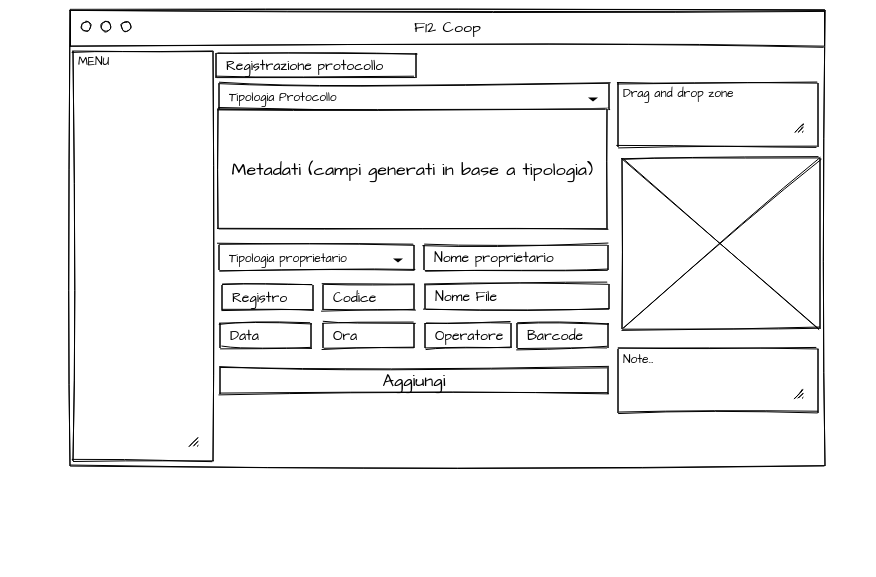
\includegraphics[width=1\columnwidth]{immagini/mockup/Registrazioneprotocollo.png} 
    \caption{Mockup - Registrazione Protocollo}
\end{figure}
\newpage

In base alla tipologia del protocollo selezionata verranno generati dei campi "metadati" con lo scopo di arricchire di informazioni il protocollo per una più facile consultazione.
\\ 
La scelta del tipo di proprietario a cui intestare il protocollo prevede la voce "nuovo contatto" che se selezionata farà comparire un form di registrazione.
\\
Una volta premuto il tasto "Aggiungi" i dati inseriti verranno salvati nelle rispettive tabelle del \textit{database}, compreso il nuovo contatto inserito.
\\
La tipologia del protocollo e i metadati saranno configurabili dall'apposito pannello descritto in "Configurazione tipologia documento".

\subsubsection{Dashboard generale}
Nella dashboard, in base all'utente che ha eseguito l'accesso, si potrà trovare l'elenco in forma tabellare di tutti i protocolli.
\\
Nell'intestazione della pagina, per facilitare l'operatore nella ricerca di specifici protocolli, saranno presenti: i campi filtrabili, un campo input che con il focus su di esso permette di filtrare i protocolli mediante scanner di barcode e un ticket promemoria che ricorda all'utente quanti protocolli deve ancora visionare.
\begin{figure}[!h] 
    \centering 
    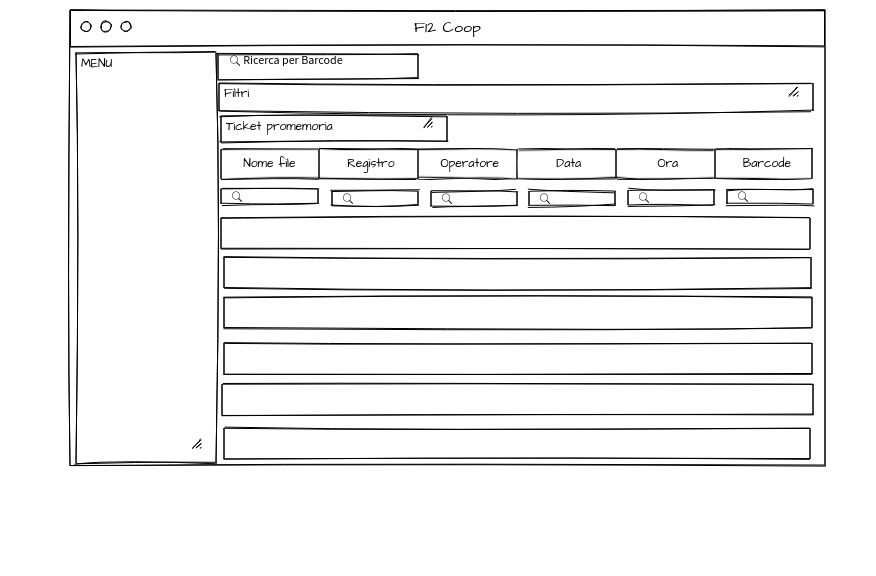
\includegraphics[width=1\columnwidth]{immagini/mockup/Dashboard.png}
    \caption{Mockup - Dashboard}
\end{figure}
\newpage

\subsubsection{Dettaglio protocollo}
Selezionando uno qualsiasi dei protocolli dalla lista precedentemente citata si aprirà la seguente pagina.
\begin{figure}[!h] 
    \centering 
    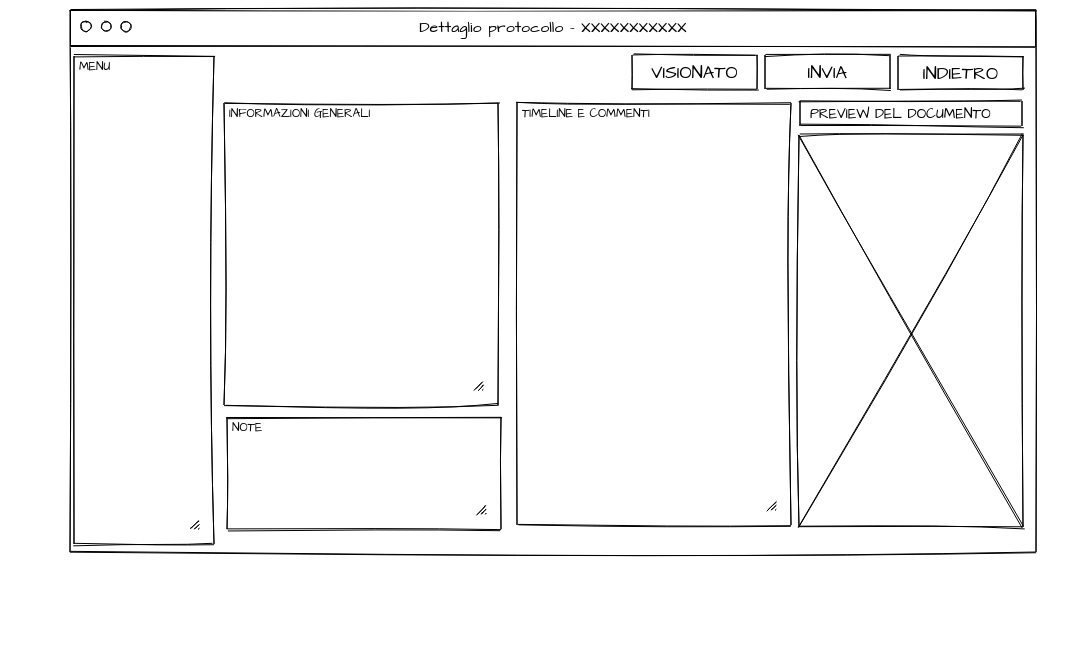
\includegraphics[width=1\columnwidth]{immagini/mockup/Editpage.png}
    \caption{Mockup - Pagina dettaglio protocollo}
\end{figure}
\\
Tra le informazioni generali, in base alla tipologia di protocollo selezionata, sarà presente la lista degli operatori addetti all'elaborazione del documento.
\\
L'utente premendo il bottone "VISIONATO" farà comparire accanto al proprio nome nella lista una spunta verde. Una volta esaminato da tutti gli operatori il protocollo sarà marcato come "visionato" e se il flusso assegnatogli lo richiede esso proseguirà con il task successivo.
\\
Premendo il tasto "INVIA" l'utente verrà rimandato ad una schermata dove è possibile compilare un form per l'invio via mail. 
\\
In fase di preparazione della e-mail verranno proposti gli indirizzi dell'intestatario del protocollo e gli indirizzi del personale interno.
\\
Nel corpo della e-mail verrà presentata una bozza di testo dove vengono riportati tutti i dati raccolti in fase di registrazione.
\\
Tra gli allegati sarà già presente il documento corrispondente al protocollo che si vuole inviare.
\\
In figura (figura 2.4), la sezione marcata come "TIMELINE E COMMENTI" ha lo scopo di far fronte all'esigenza della proponente di avere sempre visibile lo storico del protocollo. È stata inoltre aggiunta la possibilità di scrivere commenti rendendo questa sezione una vera e propria chat organizzativa.

\subsubsection{Configurazione tipologia protocollo}
Tra le voci di menù nella sezione protocolli è possibile accedere alla schermata di configurazione delle tipologie.
\begin{figure}[!h] 
    \centering 
    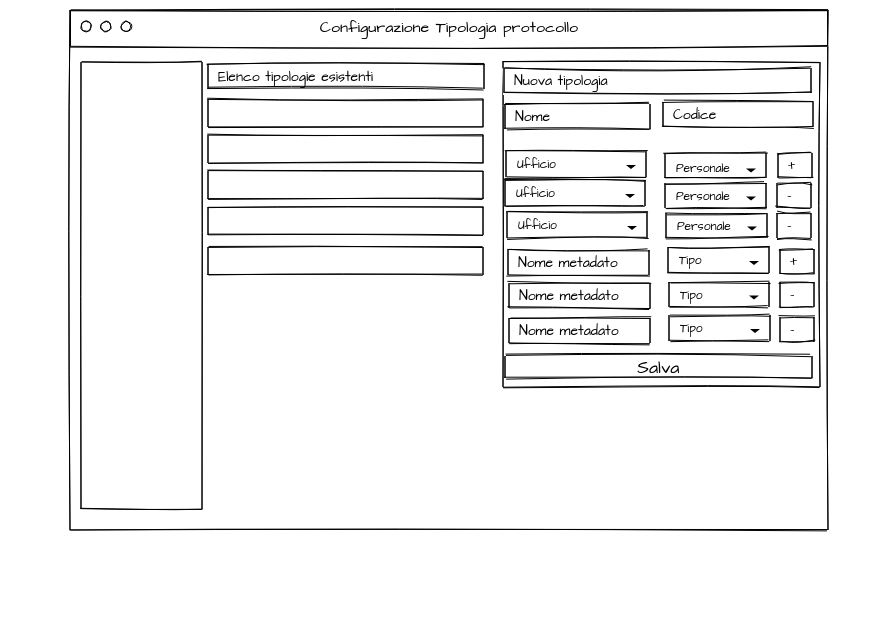
\includegraphics[width=1\columnwidth]{immagini/mockup/configtipo.png}
    \caption{Mockup - Pagina di configurazione delle tipologie}
\end{figure}
\\
La seguente maschera è pensata per far fronte all'esigenza di configurare un protocollo in base alla sua tipologia e quindi arricchirlo di informazioni utili alla facile consultazione e archiviazione. Sarà quindi possibile visionare l'elenco di tutte le tipologie di protocolli create nella lista sulla sinistra e sulla destra un semplice form per la creazione di una nuova tipologia.
\\
Come detto in precedenza, creando una nuova tipologia sarà possibile assegnare il personale addetto all'elaborazione della suddetta e sarà possibile aggiungere campi metadato.

\subsubsection{Dettaglio configurazione tipologia protocollo}
Selezionando una qualsiasi delle tipologie dalla lista precedentemente citata si aprirà la seguente pagina.
\begin{figure}[!h] 
    \centering 
    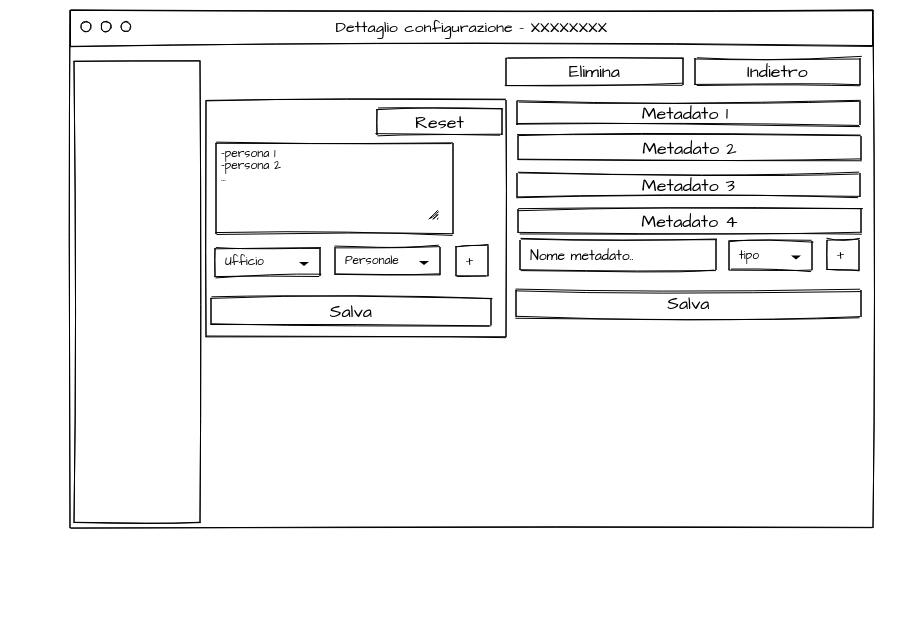
\includegraphics[width=1\columnwidth]{immagini/mockup/dettaglioconfig.png}
    \caption{Mockup - Pagina dettaglio configurazione tipologia}
\end{figure}
\\
Saranno visibili tutti i metadati e gli addetti precedentemente inseriti e sarà possibile aggiungerne di nuovi.\\
L'eliminazione di una configurazione sarà consentita solo nel caso in cui non ci saranno documenti associati alla configurazione in esame.
%**************************************************************
\newpage
\subsection{Struttura del software}
La struttura finale del software sarà la seguente.

\begin{figure}[!h] 
    \centering 
    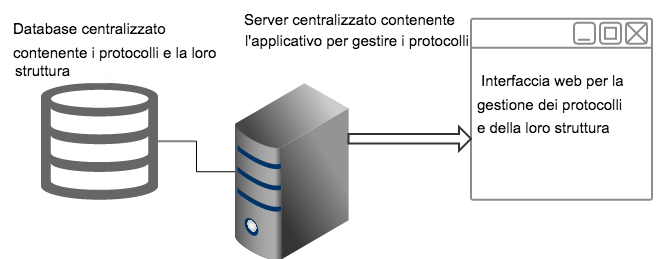
\includegraphics[width=1\columnwidth]{immagini/prodottofinito/strutturasoftware.png}
    \caption{Struttura del software}
\end{figure}

%**************************************************************